% !TeX program = xelatex
\documentclass[UTF8]{beamer}

% -----------------------------------------------------------------------------
% Language, typography, mathematics, tables, graphics
% -----------------------------------------------------------------------------
\usepackage{xeCJK}
\usepackage{amsmath}
\usepackage{physics}
\usepackage{booktabs}
\usepackage{tabularx}
\usepackage{array}
\usepackage{graphicx}
\usepackage{xcolor}
\usepackage{tcolorbox}
\tcbuselibrary{skins}
\usepackage{tikz}
\usetikzlibrary{arrows.meta,positioning,calc}

% Preserve the reusable presentation typography.
\usepackage[T1]{fontenc}
\usepackage{palatino}
\setCJKmainfont{Noto Serif CJK SC}
\setCJKsansfont{Noto Serif CJK SC}
\setCJKmonofont{Noto Serif CJK SC}
\setmonofont{Inconsolata}
\def\mathfamilydefault{\rmdefault}

% 16:9 slide canvas from the Durham/Stanford template.
\usepackage[
  orientation=landscape,
  size=custom,
  width=16,
  height=9,
  scale=0.5
]{beamerposter}

% Compatibility fix for older Babel releases.
\makeatletter
\let\@@magyar@captionfix\relax
\makeatother

% -----------------------------------------------------------------------------
% Theme and deck-specific visual language
% -----------------------------------------------------------------------------
\usetheme{Stanford}
\beamertemplatenavigationsymbolsempty
\setbeamerfont{frametitle}{size=\Large,series=\bfseries}
\setbeamerfont{title}{size=\LARGE,series=\bfseries}
\setbeamercolor{itemize item}{fg=darkcyan}
\setbeamercolor{itemize subitem}{fg=darkcyan}
\setbeamercolor{enumerate item}{fg=darkcyan}

\definecolor{planblue}{RGB}{29,78,121}
\definecolor{planteal}{RGB}{0,124,146}
\definecolor{plangreen}{RGB}{0,128,96}
\definecolor{plangold}{RGB}{188,122,25}
\definecolor{planrose}{RGB}{174,63,79}
\definecolor{planred}{RGB}{158,42,43}
\definecolor{planpale}{RGB}{244,247,249}

\newtcolorbox{phasebox}[2][]{%
  enhanced,
  colback=white,
  colframe=#2,
  boxrule=1.2pt,
  arc=1.5mm,
  left=1.6mm,
  right=1.6mm,
  top=0.9mm,
  bottom=0.9mm,
  before upper={\raggedright},
  #1
}

\newcommand{\metric}[3]{%
  \begin{tcolorbox}[
    enhanced,
    colback=#1!7,
    colframe=#1,
    boxrule=1.0pt,
    arc=1.2mm,
    left=1.8mm,
    right=1.8mm,
    top=0.5mm,
    bottom=0.5mm,
    before upper={\raggedright}
  ]
    {\color{#1}\bfseries\large #2}\hspace{1.0ex}{\footnotesize #3}
  \end{tcolorbox}%
}

\newcommand{\source}[1]{%
  \par\vfill\nointerlineskip
  \hbox to \linewidth{\hfill
    \smash{\raisebox{0pt}[0pt][0pt]{\tiny\color{coolgray}Source: #1}}}%
}

\newcommand{\Mpch}{\,h^{-1}\mathrm{Mpc}}

% -----------------------------------------------------------------------------
% Presentation metadata
% -----------------------------------------------------------------------------
\title[DEGRACE L1024 outputs]{\textbf{DEGRACE L1024 production outputs}}
\subtitle{Snapshot schedule and lens planes: what to implement in MG-GLAM}

\author[C.-Z. Ruan]{\Large Cheng-Zong Ruan}

\institute[Durham University]{%
  
\includegraphics[height=0.72in]{durham_logo.png}\\[0.65ex]
  \small Institute for Computational Cosmology, Durham University
}
\date{16 October 2026 \quad\textcolor{coolgray}{\small plan for review, nothing implemented yet}}

% -----------------------------------------------------------------------------
% Document
% -----------------------------------------------------------------------------
\begin{document}

\begin{frame}[plain]
  \titlepage
\end{frame}

% -----------------------------------------------------------------------------
\begin{frame}{Agreed on Slack: lens planes instead of particles}
  \footnotesize
  \begin{columns}[T,totalwidth=\textwidth]
    \begin{column}{0.485\textwidth}
      \begin{phasebox}[colback=planred!6,top=1.0mm,bottom=1.0mm]{planred}
        {\color{planred}\bfseries Drop particle snapshots}\par\smallskip
        $2048^3$ particles with positions and velocities: 200\,GB per snapshot,
        9\,TB per box. Not feasible for 100 LCDM boxes.
      \end{phasebox}
      \vspace{0.3ex}
      \scriptsize
      \begin{itemize}\setlength\itemsep{0.2em}
        \item \texttt{iSave=0}; checkpoints still written for restart, deleted at the end.
        \item Velocities survive only in the BDM halo catalogues (\texttt{CatshortV}).
        \item Scope: \textbf{L1024, Np2048, Ng4096}, fiducial Planck 2015, later the
              design cosmologies. Not the L1800 suite (256 does not divide 1800).
      \end{itemize}
    \end{column}
    \hfill
    \begin{column}{0.485\textwidth}
      \begin{phasebox}[colback=plangreen!6,top=1.0mm,bottom=1.0mm]{plangreen}
        {\color{plangreen}\bfseries Store projected density: lens planes}\par\smallskip
        At every output, project the density along each of the 3 axes in
        4 slabs of depth $256\Mpch$: \textbf{12 planes of $4096^2$ float32}.
      \end{phasebox}
      \vspace{0.3ex}
      \metric{plangreen}{0.8\,GB}{per snapshot (12 planes)}
      \metric{planteal}{34\,GB}{per box (42 outputs)}
      \metric{planblue}{3.4\,TB}{for 100 LCDM boxes}
    \end{column}
  \end{columns}

  \smallskip
  \begin{phasebox}[colback=planpale,top=0.6mm,bottom=0.6mm]{plangold}
    \centering\scriptsize
    \textbf{42 outputs per box} $=$ 17 \emph{primary} $z$ ($0, 0.125, \ldots, 2$; common to all cosmologies)
    $+$ 25 \emph{secondary} at $\chi = 256\,k\Mpch$, $k = 1 \ldots 25$ (FORGE / DEGRACE-ECOSMOG convention).
  \end{phasebox}
  \source{\texttt{slack-chat-degrace-prep.txt}; plan in \texttt{docs/degrace\_companion\_implementation\_plan.md}}
\end{frame}

% -----------------------------------------------------------------------------
\begin{frame}{The 42-output schedule}
  \footnotesize
  \begin{columns}[T,totalwidth=\textwidth]
    \begin{column}{0.64\textwidth}
      \centering
      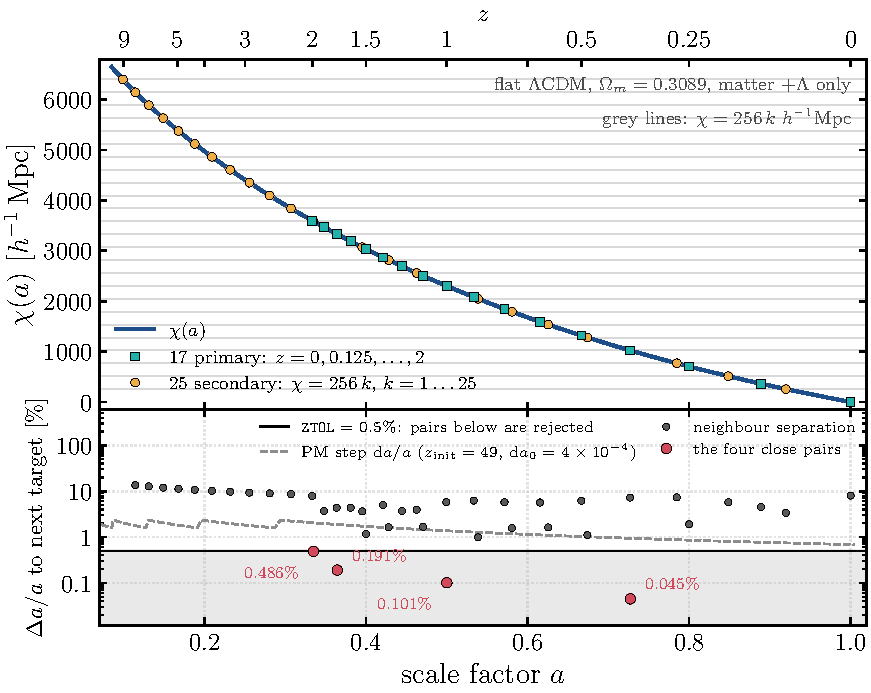
\includegraphics[width=\linewidth,height=0.76\textheight,keepaspectratio]{figs/output_schedule.pdf}
    \end{column}
    \hfill
    \begin{column}{0.34\textwidth}
      \begin{phasebox}{planblue}
        {\color{planblue}\bfseries Primary (17)}\par\smallskip
        \scriptsize
        $z = 0$ to $2$ in steps of $0.125$. Same for every cosmology; the natural
        epochs for halo catalogues and emulator training.
      \end{phasebox}
      \vspace{0.3ex}
      \begin{phasebox}{plangold}
        {\color{plangold}\bfseries Secondary (25)}\par\smallskip
        \scriptsize
        $\chi(a) = 256\,k\Mpch$, $k=1\ldots25$, out to $6400\Mpch$ ($z \simeq 9.1$).
        Cosmology dependent: recompute per design node.
      \end{phasebox}
      \vspace{0.3ex}
      \begin{phasebox}[colback=planred!5]{planred}
        {\color{planred}\bfseries Four close pairs}\par\smallskip
        \scriptsize
        Separations $0.49\%$, $0.19\%$, $0.10\%$, $0.045\%$ in $a$. The exact-$z$
        code rejects anything below $0.5\%$ (slide I1).
      \end{phasebox}
    \end{column}
  \end{columns}
  \source{\texttt{figs/make\_output\_schedule\_fig.py}; PM ladder for $z_{\rm init}=49$, $\mathrm{d}a_0 = 4\times10^{-4}$}
\end{frame}

% -----------------------------------------------------------------------------
\begin{frame}{Cross-check: Baojiu's scale factors are correct}
  \footnotesize
  Baojiu asked for an independent check of his 42 values against the Planck 2015
  parameters. Each secondary target was recomputed as the root of
  $\chi(a) = 256\,k\Mpch$ with
  $\chi(a) = \dfrac{c}{H_0}\displaystyle\int_a^1 \frac{\mathrm{d}a'}{a'^2 E(a')}$,
  $c/H_0 = 2997.92458\Mpch$.

  \medskip
  \begin{center}
    \scriptsize
    \begin{tabular}{@{}llrr@{}}
      \toprule
      background assumed & $E^2(a)$ & $\max |\Delta a / a|$ & $\Delta\chi$ at $6400\Mpch$ \\
      \midrule
      \textbf{Planck 2015, matter $+\Lambda$ only} & $0.3089\,a^{-3} + 0.6911$ & $\mathbf{7.7\times10^{-8}}$ & $< 0.001\Mpch$ \\
      plus radiation ($h=0.6774$, $N_{\rm eff}=3.046$) & $+\,\Omega_r a^{-4}$ & $1.7\times10^{-3}$ & $2.8\Mpch$ \\
      $\Omega_m = 0.3156$ instead & & $2.9\times10^{-2}$ & $49\Mpch$ \\
      \bottomrule
    \end{tabular}
  \end{center}

  \medskip
  \begin{columns}[T,totalwidth=\textwidth]
    \begin{column}{0.48\textwidth}
      \begin{phasebox}[colback=plangreen!6]{plangreen}
        {\color{plangreen}\bfseries Conclusions}\par\smallskip
        \scriptsize
        \begin{itemize}\setlength\itemsep{0.2em}
          \item The list reproduces flat $\Lambda$CDM with $\Omega_m = 0.3089$ to his integrator's noise.
          \item Distance convention is matter $+\Lambda$ only; the lightcone code must use the same $\chi(a)$.
        \end{itemize}
      \end{phasebox}
    \end{column}
    \hfill
    \begin{column}{0.48\textwidth}
      \begin{phasebox}[colback=planred!5]{planred}
        {\color{planred}\bfseries Do not reuse the Node\_082 list}\par\smallskip
        \scriptsize
        The 43-entry list read from bl267's ECOSMOG run is for the Node\_082
        cosmology (stations differ by up to $3\%$ in $a$). \texttt{ic2pm\_val\_L1024}
        used it in legacy nearest-step mode, including $z_{\rm init} = 49$.
      \end{phasebox}
    \end{column}
  \end{columns}
  \source{scipy quad/brentq, cosemu env, 2026-10-16; snippet in the markdown plan}
\end{frame}

% -----------------------------------------------------------------------------
\begin{frame}{I1 (blocker): four pairs below the $0.5\%$ tolerance}
  \footnotesize
  \begin{columns}[T,totalwidth=\textwidth]
    \begin{column}{0.47\textwidth}
      \scriptsize\setlength{\tabcolsep}{2pt}
      \begin{tabular}{@{}llrr@{}}
        \toprule
        pair ($z$) & $a$ & sep.\ in $a$ & $\Delta a$ \\
        \midrule
        2.0000 / 1.98541 & 0.33333 / 0.33496 & 0.486\% & $1.6\times10^{-3}$ \\
        1.7500 / 1.74475 & 0.36364 / 0.36433 & 0.191\% & $7.0\times10^{-4}$ \\
        1.00202 / 1.0000 & 0.49950 / 0.50000 & 0.101\% & $5.1\times10^{-4}$ \\
        0.37562 / 0.3750 & 0.72695 / 0.72727 & 0.045\% & $3.3\times10^{-4}$ \\
        \bottomrule
      \end{tabular}

      \vspace{0.8ex}
      \begin{phasebox}[colback=planpale]{planblue}
        \scriptsize
        \texttt{SetExactSteps}: a target within \texttt{ZTOL}$=0.5\%$ of a scheduled
        step \emph{moves} that step onto the target; two targets closer than
        \texttt{ZTOL} are rejected, because the second would re-move the step pinned
        to the first. Other neighbours are $\geq 0.99\%$ apart; the late-time PM step
        is $6.8\times10^{-3}$, so the closest pair is $\sim 1/20$ of a step.
      \end{phasebox}
      \vspace{0.8ex}
      \begin{phasebox}{plangold}
        {\color{plangold}\bfseries Tests} (\texttt{test/precise\_z/}, Nrow 128)\par\smallskip
        \scriptsize
        The four pairs $\rightarrow$ 42 marked steps, headers bit-exact at $1/(1+z)$,
        no duplicate step, one restart across a pinned pair; existing cases unchanged.
      \end{phasebox}
    \end{column}
    \hfill
    \begin{column}{0.5\textwidth}
      \begin{phasebox}[colback=plangreen!6]{plangreen}
        {\color{plangreen}\bfseries Proposed fix}\par\smallskip
        \scriptsize
        \begin{enumerate}\setlength\itemsep{0.3em}
          \item Never move a step that is already pinned (\texttt{MarkX=1}); insert a
                new step instead. Keep $0.5\%$ for moving \emph{unpinned} steps, so
                35 of the 42 targets still merge and only $\sim$7 PM steps are added.
          \item Relax the pair rejection to ``distinct in Real*4''
                (relative separation $> 10^{-5}$); keep the error for true duplicates.
          \item Post-conditions: all $\mathrm{d}a > 0$, \texttt{Alist} strictly increasing,
                exactly \texttt{Nexact} pinned steps, each at the Real*4 of $1/(1+z)$.
          \item Restart check unchanged (checkpoint $a$ must equal \texttt{Alist(ISTEP)}).
          \item The variable-step leapfrog already handles the short step
                ($F_V \approx 0.09$ then $\approx 1.9$ around $\Delta a = 3.3\times10^{-4}$).
        \end{enumerate}
      \end{phasebox}
    \end{column}
  \end{columns}
  \source{\texttt{PMP2main.f90} \texttt{SetExactSteps}; 244-step ladder for $z_{\rm init}=49$, $\mathrm{d}a_0=4\times10^{-4}$}
\end{frame}

% -----------------------------------------------------------------------------
\begin{frame}{I2: lens-plane output}
  \footnotesize
  \begin{columns}[T,totalwidth=\textwidth]
    \begin{column}{0.42\textwidth}
      \centering
      \begin{tikzpicture}[scale=0.46, every node/.style={font=\scriptsize}]
        \foreach \i/\c in {0/planblue,1/planteal,2/plangold,3/planrose} {
          \fill[\c!18] (\i*1.5,0) rectangle ({(\i+1)*1.5},6);
          \draw[\c,line width=0.8pt] (\i*1.5,0) rectangle ({(\i+1)*1.5},6);
        }
        \draw[|-|,coolgray] (0,-0.5) -- (6,-0.5) node[midway,below] {Box $=1024\Mpch$};
        \draw[|-|,coolgray] (0,6.4) -- (1.5,6.4) node[midway,above] {$256\Mpch$};
        \node[rotate=90] at (-0.5,3) {$4096$ cells};
        \foreach \i/\c in {0/planblue,1/planteal,2/plangold,3/planrose} {
          \draw[-{Latex[length=2mm]},coolgray] ({\i*1.5+0.75},0) -- (7.4,{5.0-\i*1.45});
          \fill[\c!30] (7.4,{4.4-\i*1.45}) rectangle (8.6,{5.6-\i*1.45});
          \draw[\c,line width=0.8pt] (7.4,{4.4-\i*1.45}) rectangle (8.6,{5.6-\i*1.45});
        }
        \node[align=center] at (8.0,-0.55) {4 planes\\$4096^2$ float32};
        \node[align=center] at (4.0,-1.7) {\textbf{$\times\,3$ axes $= 12$ planes per output}};
      \end{tikzpicture}

      \vspace{0.6ex}
      \begin{phasebox}{planteal}
        {\color{planteal}\bfseries Parameters}\par\smallskip
        \scriptsize
        Two lines \emph{appended} to \texttt{Init.dat}/\texttt{Setup.dat}, read with
        \texttt{iostat}, default off: slabs per axis (4) and plane grid (4096, must divide
        $N_{\rm grid}$). Every existing run directory stays valid.
      \end{phasebox}
    \end{column}
    \hfill
    \begin{column}{0.56\textwidth}
      \begin{phasebox}{planblue}
        {\color{planblue}\bfseries Algorithm} (generalises \texttt{ProjectDENSIT})\par\smallskip
        \scriptsize
        \begin{itemize}\setlength\itemsep{0.15em}
          \item After \texttt{DENSIT} and \textbf{before} \texttt{GetPower}, which overwrites the mesh \texttt{FI}.
          \item Per axis: slab $s = \lfloor (i-1)/(N_{\rm grid}/N_{\rm slab}) \rfloor + 1$; sum $1+\delta$ over
                the slab's cells of each column, divide by their number
                $\Rightarrow$ mean $1+\delta$ of the slab column ($\Sigma/\bar\Sigma$).
          \item OpenMP over the outer loop; extra memory $12\times4096^2\times4\,\mathrm{B} = 0.8$\,GB.
          \item Logged checks: each plane averages to 1; the 4 slabs sum to the full-box projection.
        \end{itemize}
      \end{phasebox}
      \vspace{0.3ex}
      \begin{phasebox}{plangold}
        {\color{plangold}\bfseries File} \texttt{LensPlanes.<step>.<box>.dat}, one per output\par\smallskip
        \scriptsize
        Stream access, explicit little-endian (the build is globally big-endian).
        Header: $a$, step, $N_{\rm grid}$, $N_{\rm lens}$, $N_{\rm slab}$, Box, depth,
        $\Omega_m$, $\Omega_\Lambda$, $h$. Then the 12 planes in fixed order
        X$_{1..4}$, Y$_{1..4}$, Z$_{1..4}$, each $N_{\rm lens}^2$ real*4, column-major.
        A numpy reader goes into halocat.
      \end{phasebox}
    \end{column}
  \end{columns}
  \source{\texttt{PMP2mod\_density.f90} \texttt{ProjectDENSIT}; \texttt{PMP2mod\_analyze.f90} \texttt{Analysis}; \texttt{PMP2init.f90}; \texttt{PMP2mod\_tools.f90}}
\end{frame}

% -----------------------------------------------------------------------------
\begin{frame}{I3--I6: schedule, index file, content control, config}
  \footnotesize
  \begin{columns}[T,totalwidth=\textwidth]
    \begin{column}{0.485\textwidth}
      \begin{phasebox}{planblue}
        {\color{planblue}\bfseries I3 Output schedule}\par\smallskip
        \scriptsize
        \begin{itemize}\setlength\itemsep{0.15em}
          \item \texttt{Init.dat}: \texttt{\#outputs = -42} + the 42 redshifts (exact mode).
          \item \textbf{Do not list} $z_{\rm init} = 49$: exact mode enforces $0 \le z < z_{\rm init}$;
                the IC file is the $z=49$ snapshot.
          \item Generator script: stations from $\chi(a)$ of the run's $\Omega_m$, merged with the
                17 primary $z$; must reproduce Baojiu's list to $<10^{-7}$.
        \end{itemize}
      \end{phasebox}
      \vspace{0.3ex}
      \begin{phasebox}{planteal}
        {\color{planteal}\bfseries I4 Step $\to$ redshift index}\par\smallskip
        \scriptsize
        Snapshot files are named by \texttt{ISTEP}, irregular once targets are inserted.
        Write \texttt{OutputSchedule.dat} at run start (\texttt{ISTEP a z chi exact});
        halocat loaders map snapshot numbers from it.
      \end{phasebox}
    \end{column}
    \hfill
    \begin{column}{0.485\textwidth}
      \begin{phasebox}{plangold}
        {\color{plangold}\bfseries I5 Per-output content control} (only if needed)\par\smallskip
        \scriptsize
        \texttt{iBDM}, \texttt{iPower} and the lens-plane flag are global: they fire at every
        marked step. If halo catalogues are wanted only at the 17 primary redshifts, add a
        per-redshift class consulted by the output block in \texttt{PMP2main.f90}.
        Deferred until Baojiu answers question 1.
      \end{phasebox}
      \vspace{0.3ex}
      \begin{phasebox}{plangreen}
        {\color{plangreen}\bfseries I6 Run configuration and provenance}\par\smallskip
        \scriptsize
        \begin{itemize}\setlength\itemsep{0.15em}
          \item \texttt{iSave=0}, \texttt{iPower=1}, \texttt{iBDM=1}, lens planes on.
          \item \texttt{Ncheckpoint} small enough that losing a 72\,h job does not restart from $z_{\rm init}$
                ($\sim$250 PM steps per box).
          \item Per box: \texttt{Init.dat}, \texttt{OutputSchedule.dat}, the 2LPTIC/\texttt{ic2pm}
                velocity-epoch line (\texttt{AGENTS.md}).
        \end{itemize}
      \end{phasebox}
    \end{column}
  \end{columns}
  \source{\texttt{PMP2init.f90} parser; limits \texttt{zout(1000)}, \texttt{NstepM=2000}}
\end{frame}

% -----------------------------------------------------------------------------
\begin{frame}{Disk budget per box and open questions for Baojiu}
  \footnotesize
  \begin{columns}[T,totalwidth=\textwidth]
    \begin{column}{0.55\textwidth}
      \scriptsize\setlength{\tabcolsep}{3pt}
      \begin{tabular}{@{}lrrr@{}}
        \toprule
        product & per snapshot & per box & 100 boxes \\
        \midrule
        lens planes ($12\times4096^2$ float32) & 0.8\,GB & 34\,GB & 3.4\,TB \\
        \texttt{CatshortV} catalogues$^\dagger$ & 0.3--0.4\,GB & $\sim$15\,GB & $\sim$1.5\,TB \\
        \texttt{PowerDM} & kB & -- & -- \\
        particle snapshots (\texttt{iSave=1}) & 200\,GB & 8.4\,TB & no \\
        \texttt{PMcrs} checkpoints (transient) & 200\,GB & 200\,GB & deleted \\
        \bottomrule
      \end{tabular}
      \par\smallskip
      $^\dagger$ pilot model65 box 1, \texttt{MassMin}$=5\times10^{11}$, if BDM runs at all 42 outputs.
    \end{column}
    \hfill
    \begin{column}{0.42\textwidth}
      \begin{phasebox}[colback=planpale]{plangold}
        {\color{plangold}\bfseries Open questions}\par\smallskip
        \scriptsize
        \begin{enumerate}\setlength\itemsep{0.3em}
          \item BDM catalogues at all 42 outputs, or only at the 17 primary redshifts?
          \item Lens planes at the primary redshifts too, or only at the 26 stations
                ($z=0$ and $k=1\ldots25$)? His 34\,GB assumes all 42.
          \item Plane normalisation: mean $1+\delta$ of the slab column (proposed) or surface density?
                Must match his ECOSMOG planes.
          \item Keep the four close pairs (fix I1) or drop one of each? They differ by $\le 1.5\Mpch$ in $\chi$.
        \end{enumerate}
      \end{phasebox}
    \end{column}
  \end{columns}
  \source{pilot model65 box 1, \texttt{Run1/CATALOGS}}
\end{frame}

% -----------------------------------------------------------------------------
\begin{frame}{Summary and next steps}
  \footnotesize
  \begin{columns}[T,totalwidth=\textwidth]
    \begin{column}{0.48\textwidth}
      \begin{phasebox}[colback=plangreen!6]{plangreen}
        {\color{plangreen}\bfseries Done}\par\smallskip
        \begin{itemize}\setlength\itemsep{0.2em}
          \item Baojiu's 42 scale factors verified against Planck 2015 (matter $+\Lambda$).
          \item Existing code located: exact-$z$ scheduler, \texttt{ProjectDENSIT}, output block.
          \item Plan written: \texttt{docs/degrace\_lensplanes\_}\\\texttt{implementation\_plan.md}.
        \end{itemize}
      \end{phasebox}
      \vspace{0.4ex}
      \begin{phasebox}[colback=planred!5]{planred}
        {\color{planred}\bfseries Blocker}\par\smallskip
        I1: the $0.5\%$ pair rejection in \texttt{SetExactSteps} refuses Baojiu's list as is.
      \end{phasebox}
    \end{column}
    \hfill
    \begin{column}{0.48\textwidth}
      \begin{phasebox}{planblue}
        {\color{planblue}\bfseries Order of work} (branch off \texttt{cz})\par\smallskip
        \begin{enumerate}\setlength\itemsep{0.2em}
          \item Reply to Baojiu: cross-check result, questions 1--4.
          \item I1 pinned-step fix + \texttt{test/precise\_z} cases.
          \item I2 lens planes: routine, parameters, file format, numpy reader.
          \item I3 schedule generator; I4 \texttt{OutputSchedule.dat}.
          \item I5 only if question 1 says ``primary only''.
          \item Pilot one L1024 box with the full 42-output schedule; check
                efficiency and sizes before the 100-box campaign.
        \end{enumerate}
      \end{phasebox}
    \end{column}
  \end{columns}
  \vfill
  \centering
  \textbf{Everything above is a proposal for review; no source has been changed.}
\end{frame}

\end{document}
